%% BidSense --- IEEE conference format (IEEEtran).
%%
%% Compile: pdflatex bidsense && bibtex bidsense && pdflatex bidsense
%% Overleaf: upload this file, select pdfLaTeX. IEEEtran.cls ships with Overleaf.
%%
%% EVERY number in Section V is produced by a named script in backend/scripts/.
%% Figures marked [PENDING] are measured by an instrument that exists but
%% requires the corpus restored and an LLM provider with quota; they are flagged
%% in the text rather than filled with a plausible value.

\documentclass[conference]{IEEEtran}
\IEEEoverridecommandlockouts

\usepackage{cite}
\usepackage{amsmath,amssymb}
\usepackage{graphicx}
\usepackage{booktabs}
\usepackage{tikz}
\usetikzlibrary{arrows.meta,positioning,fit,backgrounds}
\usepackage{xcolor}
\usepackage[hidelinks]{hyperref}

\def\BibTeX{{\rm B\kern-.05em{\sc i\kern-.025em b}\kern-.08em T\kern-.1667em\lower.7ex\hbox{E}\kern-.125emX}}

\begin{document}

\title{Where to Stop Using a Language Model:\\
A Deterministic Compliance Engine with\\
LLM-Located Evidence for Tender Evaluation}

\author{\IEEEauthorblockN{Dhruv Reddy Sripathi}
\IEEEauthorblockA{\textit{Department of Computer Science and Engineering}\\
\textit{[Institution]}\\
[City], India \\
sdvjmchatgpt@gmail.com}
}

\maketitle

\begin{abstract}
Public tender evaluation requires deciding whether a bid satisfies every
mandatory eligibility criterion and encloses every mandatory document, and
requires citing the specific clause behind each decision, because a bidder may
challenge it. Retrieval-augmented generation is an obvious fit for the reading
task and a poor fit for the deciding one. We present BidSense, a system that
partitions the problem: a language model locates and cites evidence in the
source documents, and a deterministic rule engine makes every disqualifying
decision. We argue the partition is not merely conservative engineering but
empirically necessary, and we build the instrument to test it --- an LLM-only
elimination baseline scored by the same clause comparator as the rule engine, on
the same labelled bids. Our contributions are: (i) the architectural partition
and its audit trail, in which no document is ever declared present on a
sub-threshold match; (ii) a measured retrieval result showing that chunking
table rows individually, rather than appending tables to page prose, moves a
dense retriever from \emph{worse} than BM25 (hit@1 5.9\%) to clearly better
(47.1\%), a difference significant under an exact paired sign test; (iii) an
evaluation methodology for small corpora in which every proportion carries a
Wilson interval and every arm-to-arm comparison is paired, which we show is
necessary by exhibiting a clean five-nil sweep that does not reach
$p<0.05$; and (iv) a candid account of the validity threats that remain,
principally the synthetic provenance of the bid corpus. We report what is
measured, mark what is not, and state the sample size behind every figure.
\end{abstract}

\begin{IEEEkeywords}
retrieval-augmented generation, document understanding, compliance checking,
public procurement, information extraction, evaluation methodology
\end{IEEEkeywords}

\section{Introduction}

A public tender notification is a long, structurally irregular document --- in
our corpus, 56 to 382 pages --- that states eligibility criteria, mandatory
enclosures, deadlines and financial thresholds. A bid is a second long document
that claims to satisfy them. Technical evaluation is the act of deciding, for
every requirement, whether the bid meets it, and of recording why.

Two properties make this task unusual for a language-model pipeline.

First, \textbf{the citation is part of the answer}. A procurement committee that
eliminates a bidder must be able to name the clause relied upon. An evaluation
that reaches the correct verdict while citing the wrong clause is not a partially
correct answer; it is an indefensible decision. Standard
retrieval-augmented generation \cite{lewis2020rag} is evaluated predominantly on
answer correctness, where a fluent answer supported by \emph{some} retrieved
passage scores well.

Second, \textbf{the decision rule is already written down}. Unlike open-domain
question answering, the criteria are explicit in the tender: a turnover floor, a
similar-work threshold, a list of documents. Once the values are extracted, the
decision is arithmetic and set membership. A model asked to perform that
arithmetic is doing work that cannot be audited, and doing it less reliably than
a comparison operator.

These two observations motivate a partition. BidSense uses a language model for
what language models are good at --- reading irregular layout, resolving that
``earnest money'' and ``EMD'' denote the same obligation, locating the page a
figure sits on --- and a deterministic engine for every decision that eliminates
a bidder. The contribution of this paper is not the partition as an idea, which
is folklore in applied information-extraction pipelines \cite{rashkin2023ais},
but the measurement of where the boundary must fall and what is lost by moving
it.

\subsection{Contributions}

\begin{enumerate}
  \item An architecture that separates evidence location from adjudication,
  with a four-tier document-name matcher that distinguishes \textsc{present},
  \textsc{missing} and \textsc{needs-review}, and never declares a document
  present on a sub-threshold similarity score (Section~\ref{sec:method}).
  \item A retrieval finding obtained by ablation on identical labels: chunking
  table rows individually moves dense retrieval from below a BM25 baseline to
  clearly above it. Before the change the dense retriever was worse than
  keyword search on every metric (Section~\ref{sec:results}).
  \item An evaluation methodology for small labelled corpora: Wilson intervals
  on every proportion, exact paired sign tests for hit@$k$, and a seeded
  percentile bootstrap for MRR. We show this is not pedantry by exhibiting a
  five-improved/zero-regressed sweep with $p=0.0625$
  (Section~\ref{sec:method-eval}).
  \item An instrument for the central claim --- an LLM-only elimination
  baseline --- together with an explicit statement of the sample size at which
  that claim becomes provable, which our present corpus does not reach
  (Sections~\ref{sec:results} and \ref{sec:threats}).
\end{enumerate}

\section{Related Work}
\label{sec:related}

\textbf{Retrieval-augmented generation.} Lewis \textit{et al.}
\cite{lewis2020rag} pair a sequence-to-sequence generator with a dense index
queried by a neural retriever. We adopt this architecture for the
question-answering path and depart from its evaluation posture: because the
cited clause is itself the deliverable, we measure citation faithfulness
separately from answer correctness rather than reporting a single score.

\textbf{Dense versus sparse retrieval.} Karpukhin \textit{et al.}
\cite{karpukhin2020dpr} show a dual-encoder retriever outperforming Lucene-BM25
by 9--19 points of top-20 accuracy. Robertson and Zaragoza \cite{robertson2009bm25}
survey the probabilistic relevance framework from which BM25 derives. We use
BM25 as a baseline rather than a straw man: tender documents are dense with
exact figures and clause numbers, which is lexical matching's strongest ground,
and Section~\ref{sec:results} reports a configuration in which BM25 won.

\textbf{Embedding model.} We retrieve with BGE \cite{xiao2023cpack}, run
locally. The choice is driven by confidentiality as much as quality: a tender
under evaluation is commercially sensitive, and a hosted embedding API would
require transmitting bid contents to a third party.

\textbf{Clause-level understanding of contractual documents.} CUAD
\cite{hendrycks2021cuad} provides 13{,}000+ expert annotations over 510
commercial contracts across 41 clause categories, framed as surfacing the
passages a human reviewer should read rather than replacing the reviewer. This
is the nearest well-established neighbour to our task and the posture we adopt.
Two differences shape our method: CUAD identifies clause categories \emph{within}
one document, whereas tender evaluation checks a bid against the requirements of
a \emph{different} document, so the unit of judgement is a
(requirement, response) pair rather than a span.

\textbf{Attribution.} Rashkin \textit{et al.} \cite{rashkin2023ais} define
Attributable to Identified Sources (AIS), judging whether a statement can be
justified as ``According to $P$, $s$''. This is the standard our
citation-faithfulness evaluation is built against, and it is what separates the
two numbers we report for the elimination baseline.

\textbf{Agreement.} Cohen's $\kappa$ \cite{cohen1960kappa} corrects observed
agreement for chance; Landis and Koch \cite{landis1977agreement} supply the
interpretation bands we quote, which are a widely used heuristic rather than a
principled cutoff.

\textbf{Gap.} We are not aware of a verified peer-reviewed anchor for
retrieval-augmented \emph{procurement} compliance checking specifically. Several
candidates exist in the recent literature but we were unable to verify them
against their publishers of record at the time of writing, and we therefore do
not cite them. We position this work as adjacent to legal-contract NLP rather
than within an established procurement literature, and we flag
table-structure-aware retrieval as the most relevant unsurveyed neighbour, since
our table-row chunking result lies in that area.

\section{System Design}
\label{sec:method}

\begin{figure*}[t]
\centering
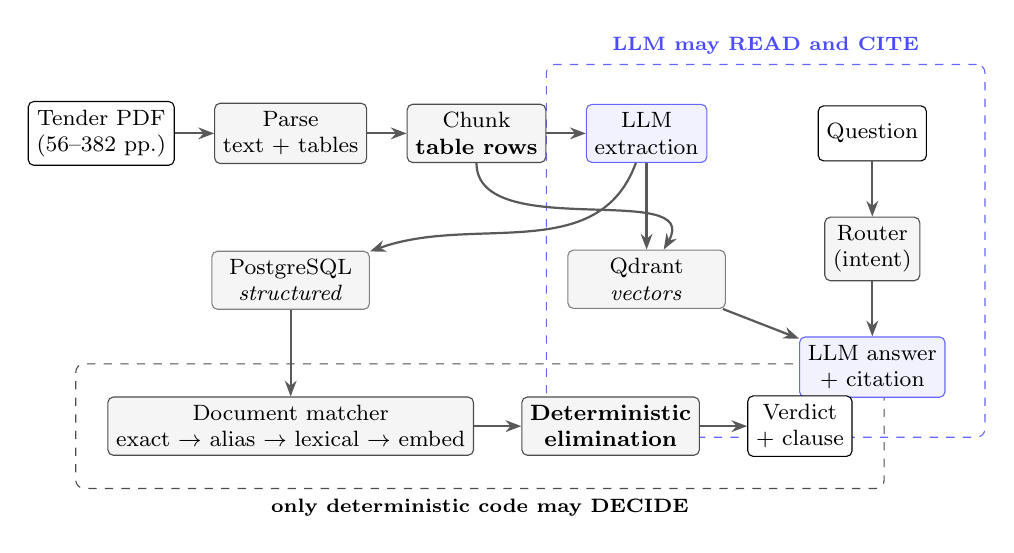
\begin{tikzpicture}[
  font=\footnotesize,
  box/.style={draw, rounded corners=2pt, minimum height=7mm, align=center,
              inner sep=3pt, fill=white},
  llm/.style={box, draw=blue!60, fill=blue!5},
  det/.style={box, draw=black!70, fill=black!4},
  store/.style={box, draw=black!50, fill=gray!8, minimum width=20mm},
  >={Stealth[length=2mm]},
  arr/.style={->, thick, draw=black!65},
]
% ingestion
\node[box] (pdf) {Tender PDF\\(56--382 pp.)};
\node[det, right=5mm of pdf] (parse) {Parse\\text + tables};
\node[det, right=5mm of parse] (chunk) {Chunk\\\textbf{table rows}};
\node[llm, right=5mm of chunk] (extract) {LLM\\extraction};

% stores
\node[store, below=11mm of parse] (pg) {PostgreSQL\\\emph{structured}};
\node[store, below=11mm of extract] (qd) {Qdrant\\\emph{vectors}};

% query path
\node[box, right=14mm of extract] (q) {Question};
\node[det, below=7mm of q] (router) {Router\\(intent)};
\node[llm, below=7mm of router] (answer) {LLM answer\\+ citation};

% decision path
\node[det, below=11mm of pg] (match) {Document matcher\\exact $\to$ alias $\to$ lexical $\to$ embed};
\node[det, right=6mm of match] (rules) {\textbf{Deterministic}\\\textbf{elimination}};
\node[box, right=6mm of rules] (out) {Verdict\\+ clause};

\draw[arr] (pdf) -- (parse);
\draw[arr] (parse) -- (chunk);
\draw[arr] (chunk) -- (extract);
\draw[arr] (extract) -- (qd);
\draw[arr] (extract) to[out=250,in=20] (pg);
\draw[arr] (chunk) to[out=270,in=60] (qd);
\draw[arr] (q) -- (router);
\draw[arr] (router) -- (answer);
\draw[arr] (qd) -- (answer);
\draw[arr] (pg) -- (match);
\draw[arr] (match) -- (rules);
\draw[arr] (rules) -- (out);

% the boundary that is the paper's argument
\begin{scope}[on background layer]
  \node[draw=blue!60, dashed, rounded corners=3pt, inner sep=5mm,
        fit=(extract)(answer), label={[blue!70, font=\scriptsize\bfseries]above:%
        LLM may READ and CITE}] {};
  \node[draw=black!70, dashed, rounded corners=3pt, inner sep=4mm,
        fit=(match)(rules)(out), label={[font=\scriptsize\bfseries]below:%
        only deterministic code may DECIDE}] {};
\end{scope}
\end{tikzpicture}
\caption{BidSense. The language model reads irregular layout and attaches
citations; it never adjudicates. Every decision that eliminates a bidder is
taken by deterministic code over values already extracted, so the decision can
be replayed and the clause behind it named. Section~\ref{sec:results} reports
what happens when the boundary is moved.}
\label{fig:arch}
\end{figure*}

Figure~\ref{fig:arch} shows the system. We describe only the components the
evaluation exercises.

\subsection{Ingestion and table-row chunking}

Documents are parsed to per-page text plus extracted tables. Eligibility data in
tenders lives overwhelmingly in tables --- a turnover floor is a cell, not a
sentence --- and our initial implementation appended a page's tables to its prose
and split the result by size. This is the configuration
Section~\ref{sec:results} shows to be worse than keyword search.

We instead emit \emph{one chunk per table row}, carrying the row's own page and
clause anchor. A row such as \texttt{11. | emd @ 1\% | rs. 2,98,720.00} becomes a
retrievable unit whose embedding is dominated by the fact it states, rather than
diluted across a page of surrounding prose.

Parsing dominates ingestion cost. Profiled on a 172-page document, parsing
accounts for 99.9\% of pipeline time (14{,}890\,ms, against 11\,ms for
chunking), and within parsing the text-based table-detection fallback is 55.8\%
at roughly 58\,ms per page on which it runs. We retain it: it is what finds the
43 tables in that document. Parsing is CPU-bound and page ranges are
independent, so we parallelise across them, measuring $2.41\times$ at four
workers with an identical SHA-256 over all extracted text and tables.

\subsection{Scoped retrieval}

Retrieval is scoped by metadata \emph{before} the vector search, not filtered
after it. Answering a question about tender $A$ with a clause from tender $B$ is
a wrong answer that looks well cited; and a post-filter leaks information
through score ordering and result counts, which matters because one bidder must
not learn anything about another's submission.

\subsection{Query-side vocabulary expansion}

Tenders write ``EMD''; bidders ask about ``earnest money''. Measured against a
real chunk, the long form costs 0.18 cosine similarity (0.4621 versus 0.6429),
enough to move the correct chunk from rank 1 to rank 193 of 388. We expand the
\emph{query} against a curated glossary of Indian procurement terms.

Two design choices are deliberate. We do not rewrite indexed text, although it
works comparably (0.4621 $\to$ 0.6310): citation highlighting matches the stored
snippet against words on the source page, so editing what we store to improve
retrieval would degrade the provenance the product rests on. And we use a
lookup rather than a model, because a wrong expansion measurably hurts ---
appending ``EMD'' to a deadline question moved the correct chunk from 0.6941 to
0.6090 --- so terms are expanded only when actually present.

\subsection{Document-name matching}

The same document is named differently in a tender and a bid (``GST
Registration Certificate'' versus ``Goods \& Services Tax Certificate''). We
match in four tiers, cheapest first, recording which tier fired so the audit
trail can show why a document counted as present: exact (normalised), alias (a
curated table of standard Indian tender documents), lexical (synonym vocabulary
plus agreement on identifying words), and finally BGE cosine similarity.

The alias table exists because embeddings are unreliable on short, jargon-heavy
strings: ``PAN Card'' and ``TAN Certificate'' are lexically and semantically
close and are entirely different documents. The lexical tier exists because of
the converse failure, measured on the real corpus: requirement names are often
sentences (``Certificate from the chartered accountant''), and a bid restating
one in ordinary vocabulary (``\dots from the statutory auditor'') scores 0.83,
below the threshold at which we are willing to declare a document present.

Below that floor we return a third answer. \textsc{needs-review} names the
near-miss candidate instead of reporting \textsc{missing} and sending a bidder
to obtain a document already in their bid under another name. \textbf{No tier
ever declares a document present on a sub-threshold score}; the review band
changes only what a failure to match is permitted to claim.

\subsection{Deterministic elimination, split by ground}

Two kinds of failure disqualify: an eligibility \emph{criterion} the bidder does
not meet, and a mandatory \emph{document} not enclosed. The engine records which
fired, for two reasons.

\textit{Curability.} A turnover shortfall cannot be remedied before the
deadline; an absent covering letter usually can. A single undifferentiated
``eliminated'' tells a bidder nothing about whether to withdraw or to file a
document.

\textit{Measurement.} The two grounds have very different accuracy, and
Section~\ref{sec:results} shows that blending them misattributed every error in
the system to the wrong component.

\section{Evaluation Methodology}
\label{sec:method-eval}

Our labelled corpus is small --- four real tender notifications across three
sectors, 19 labelled bids, 17 labelled retrieval queries --- and we treat that
as a methodological constraint rather than a footnote.

\subsection{Intervals, not bare proportions}

``100\%'' from 17 trials and ``100\%'' from 2{,}000 are different claims. Every
proportion we report carries a 95\% Wilson score interval. Wilson rather than
the normal approximation because the latter is worst exactly where this work
lives: at $n<40$ and at proportions near 0 or 1, where it produces bounds
outside $[0,1]$ and collapses to zero width at $p=1$. Accordingly, our 100\%
extraction figure is reported as $[81.6, 100.0]$ --- a reader may reasonably
read it as ``possibly 82\%''.

\subsection{Paired comparisons}

Every arm is scored on the \emph{same} queries, so comparing two arms by
overlapping intervals discards the pairing that makes the comparison sensitive.
A query both arms answer correctly carries no information about which is better;
only the queries they disagree on do. We therefore use:

\begin{itemize}
  \item an \textbf{exact two-sided sign test} (McNemar's exact test) over
  discordant queries for hit@$k$, exact rather than normal-approximate because
  $n$ is small enough that the approximation is wrong here;
  \item a \textbf{percentile bootstrap} over paired per-query deltas for MRR,
  10{,}000 resamples, seed recorded in the run manifest, because the deltas are
  a spike at zero with a few large jumps and are nowhere near normal.
\end{itemize}

This distinction is load-bearing at our $n$. A clean six-improved /
zero-regressed sweep gives $p=0.0312$ and clears $0.05$; a clean five-nil sweep
gives $p=0.0625$ and does not. We report the second as not significant
(Section~\ref{sec:results}) rather than as a win.

\subsection{Like-for-like arms in one process}

Arms are scored in a single process over identical chunks and labels. Quoting a
baseline from one script run and the treatment from a separate later run silently
credits the treatment with any label correction or code change made in between
--- a substitution we were able to make inadvertently once, and now prevent
structurally.

\subsection{Reproducibility}

A single entry point runs every evaluator and writes one result file beside a
manifest recording the git revision (flagged when the working tree is dirty),
dependency versions, the random seed, SHA-256 of every source and label file,
and the $n$ behind each figure. A stage whose prerequisites are absent is
reported \textsc{blocked} with the specific reason and no number is produced for
it, so a partial run cannot be misread as a complete one.

\section{Results}
\label{sec:results}

All figures below were produced by named scripts in \texttt{backend/scripts/}.

\subsection{Retrieval and the chunking ablation}

Table~\ref{tab:retrieval} reports both arms over the same 17 labelled queries
and the same chunks. Questions were deliberately written to avoid the documents'
own wording (``How much do I have to deposit upfront?'' rather than quoting
``Earnest Money Deposit of Rs.\ 31,500''), which handicaps a lexical method;
BM25 should therefore be read as the floor a semantic retriever must clear.

\begin{table}[htbp]
\caption{Retrieval, 17 labelled queries, four real tenders}
\label{tab:retrieval}
\centering
\begin{tabular}{@{}lrrrr@{}}
\toprule
 & hit@1 & hit@3 & hit@5 & MRR \\
\midrule
BM25 keyword baseline            & 17.6\% & 35.3\% & 47.1\% & 0.294 \\
Dense, size-split chunks         & \phantom{0}5.9\% & 17.6\% & 35.3\% & 0.149 \\
Dense, table rows chunked        & 41.2\% & 58.8\% & 64.7\% & 0.502 \\
\textbf{Dense, rows + expansion} & \textbf{47.1\%} & \textbf{64.7\%} & \textbf{70.6\%} & \textbf{0.571} \\
\bottomrule
\end{tabular}
\end{table}

The second row is the uncomfortable one and we report it deliberately: with
size-split chunks the dense retriever was \emph{worse than keyword search on
every metric}. That ordering was discovered by measuring, not by assuming, and
it is the strongest evidence we have that the table-row result is a real effect
rather than a tuning artefact.

Under the paired tests of Section~\ref{sec:method-eval}, the chunking change is
significant on hit@1 (6 improved, 0 regressed, $p=0.0312$) and on MRR, and
\emph{not} significant on hit@5 (5 improved, 0 regressed, $p=0.0625$). We state
the second as a non-result. It is also the clearest possible argument for
enlarging the query set: the effect is almost certainly real and our $n$ cannot
demonstrate it.

\subsection{Elimination, split by ground}

\begin{table}[htbp]
\caption{Elimination accuracy by ground, 19 labelled bids}
\label{tab:elim}
\centering
\begin{tabular}{@{}lrrrrr@{}}
\toprule
ground & precision & recall & TP & FP & FN \\
\midrule
criteria (threshold/status) & \textbf{100\%} & \textbf{100\%} & 6 & 0 & 0 \\
document (missing enclosure) & 60\% & 100\% & 6 & 4 & 0 \\
blended (as previously reported) & 75\% & 100\% & 12 & 4 & 0 \\
\bottomrule
\end{tabular}
\end{table}

The deterministic rule engine is exact on criteria: no compliant bidder fails a
criterion and every bidder who should fail one does. The blended 75\% figure
implicated that engine and it was not at fault --- all four false positives are
document matching, where a bid's enclosure list is compared against a 39-to-47
item checklist. We regard this as the practical argument for splitting the
ground: an aggregate metric misattributed every error in the system to the
wrong component.

Inspection of the four false positives found one genuine matcher miss
(``compliance \emph{sheet}'' versus ``clause-wise compliance \emph{statement}'',
0.614, below the 0.72 floor) and three documents the generated bids genuinely do
not contain. The correct fix is to the corpus, not the matcher, and we did not
loosen the threshold until the numbers agreed.

\subsection{The LLM-only elimination baseline}

This is the paper's central comparison and we report it as \textbf{[PENDING]}.
The instrument exists (\texttt{scripts/baseline\_elimination.py}), is unit
tested, and scores both arms on the same bids with the same clause comparator
imported from the rule-arm evaluator. Executing it requires the corpus ingested
and an LLM provider with quota, neither of which was available at the time of
writing.

We state in advance the sample size at which the claim becomes provable, so that
the result cannot be reported selectively afterwards. Reason accuracy is
judgeable only on eliminated bids whose answer key names a clause. An exact
paired sign test requires six discordant pairs before even a unanimous outcome
reaches $p=0.0312$; at three discordant pairs a clean sweep gives $p=0.2500$.
An earlier informal run of this comparison on four bids therefore could not have
supported the claim whatever it showed, and we do not report its numbers.

\subsection{Remaining measures}

\begin{table}[htbp]
\caption{All reported metrics with sample sizes}
\label{tab:all}
\centering
\begin{tabular}{@{}llr@{}}
\toprule
Metric & Result (95\% Wilson) & $n$ \\
\midrule
Extraction field accuracy & 100.0\% [81.6--100.0] & 17 fields \\
Elimination precision (criteria) & 100\% & 6 bids \\
Retrieval hit@1 & 47.1\% [26.2--69.0] & 17 queries \\
Retrieval hit@5 & 70.6\% [46.9--86.7] & 17 queries \\
Citation page truthfulness & 100\% & 31 citations \\
Router accuracy (held out) & 95.5\% [78.2--99.2] & 22 queries \\
Inter-annotator $\kappa$ & \textbf{[PENDING]} & --- \\
LLM-only baseline & \textbf{[PENDING]} & --- \\
\bottomrule
\end{tabular}
\end{table}

Router vocabulary was fitted on a development split; only the held-out figure is
evidence, and the development figure (96.4\%) measures fitting.

\section{Threats to Validity}
\label{sec:threats}

We consider the first of these decisive enough that it constrains what the paper
is entitled to claim.

\subsection{The bid corpus is synthetic}

All 19 labelled bids were generated by this project's own code from the same
tender profiles whose requirements the matcher is checked against. This is
circular in a way that directly inflates the elimination results: the generator
and the evaluator share assumptions about how a document is named and what a
compliant bid contains.

We mitigate it and do not claim to remove it. Bids restate required document
names the way a bidder would rather than copying the tender's wording, so the
alias, lexical and embedding tiers must earn their matches rather than
succeeding by string equality; and the compliance outcome of each bid is fixed
\emph{before} its prose is generated, so the answer key is a specification
rather than a post-hoc label. Mitigation is not elimination. \textbf{No real
bid has been evaluated.} Obtaining even a small number of genuine bids is the
single highest-value next step for this work, and until then the elimination
figures should be read as an upper bound obtained under favourable conditions.

\subsection{Sample size}

Seventeen retrieval queries, 17 extraction fields, 19 bids, four tenders. Every
interval in Table~\ref{tab:all} is wide and the 100\% figures have lower bounds
near 80\%. One of our own headline comparisons fails to reach significance for
this reason alone. More labelled data, not more features, is the highest-value
engineering direction.

\subsection{Label reliability is unquantified}

Every figure is measured against hand-written labels, which makes label
reliability part of the method. We built the instrument --- a blinded
double-labelling harness withholding both the recorded label and the reason text
that implies it, with Cohen's $\kappa$ and an adjudication report --- and we
deliberately report \textbf{no $\kappa$ figure}. $\kappa$ requires an
independent second rater; a second pass by the author reproduces the author's
own reading of an ambiguous clause and reports that consistency as reliability.
The harness and protocol are the contribution here; the figure requires a second
person.

\subsection{Generalisation}

One jurisdiction, one language register (Indian English public procurement),
three sectors, four documents. The alias table and the vocabulary glossary are
explicitly specific to Indian tender conventions and would need rebuilding
elsewhere. We make no cross-jurisdiction claim.

\subsection{No expert validation}

No procurement professional has assessed whether the gap reports the system
produces would be acted upon. For an applied system this is a substantive gap,
and a qualitative study with even a small number of practitioners would
materially strengthen the work.

\subsection{Artefact availability}

The source tender PDFs are large public downloads and are tracked as metadata
rather than committed. At the time of writing their source portals are recorded
as unconfirmed, which means the primary data cannot currently be re-obtained by
a third party. We regard this as a defect of the artefact independent of the
results and are addressing it with a checksum-verified fetch manifest.

\subsection{Measurement bugs found in our own evaluation}

We record these because an evaluation audited only when it flatters the author
is not an evaluation. Two bugs made the system look worse than it is: clause
references were compared literally, so a key's \texttt{1.1(4)} did not match a
cited \texttt{1.1 (4)}, scoring five correct citations as wrong and reporting
reason accuracy at 58\% instead of 75\%; and citation page-truthfulness compared
a table rendered as \texttt{Label | Value} against a running-text rendering of
the same page, scoring 50\% where the true figure was 31/31. One bug ran the
other way: two retrieval labels were wrong in a manner that understated
retrieval, and were corrected, with five genuine misses left scored as misses.
Separately, regenerating the bid corpus silently destroyed part of the answer
key --- four rows and an entire label column --- for a period during which the
evaluation measured whatever survived.

\section{Conclusion}

We have argued, and built the instrument to test, that tender compliance
evaluation should partition at the boundary between reading and deciding: a
language model may locate and cite evidence, and only deterministic code may
eliminate a bidder. The supporting evidence is a deterministic engine that is
exact on eligibility criteria across our labelled set, a retrieval improvement
from table-row chunking that is significant under a paired exact test, and an
evaluation methodology that makes the limits of a small corpus explicit rather
than incidental.

The honest summary of the work's status is that the architecture is built and
measured, while the two results that would make the central claim decisive --- an
LLM-only baseline over enough bids to reach significance, and an
inter-annotator agreement figure --- have instruments but not yet numbers, and
the bid corpus remains synthetic. We have stated which figures are pending, the
sample size each requires, and why we prefer to publish the gap rather than fill
it.

\section*{Reproducibility}

Source, evaluation scripts and the labelled answer key are in the project
repository. \texttt{python -m scripts.evaluate\_all} runs every evaluator and
emits a manifest with the git revision, dependency versions, random seed and
SHA-256 of every input. Stages whose prerequisites are absent report
\textsc{blocked} rather than a number.

\begin{thebibliography}{00}

\bibitem{lewis2020rag} P. Lewis \textit{et al.}, ``Retrieval-augmented
generation for knowledge-intensive NLP tasks,'' in \textit{Advances in Neural
Information Processing Systems 33}, 2020.

\bibitem{karpukhin2020dpr} V. Karpukhin \textit{et al.}, ``Dense passage
retrieval for open-domain question answering,'' in \textit{Proc. EMNLP}, 2020,
pp. 6769--6781.

\bibitem{robertson2009bm25} S. Robertson and H. Zaragoza, ``The probabilistic
relevance framework: BM25 and beyond,'' \textit{Foundations and Trends in
Information Retrieval}, vol. 3, no. 4, pp. 333--389, 2009.

\bibitem{xiao2023cpack} S. Xiao, Z. Liu, P. Zhang, N. Muennighoff, D. Lian, and
J.-Y. Nie, ``C-Pack: Packed resources for general Chinese embeddings,''
\textit{arXiv:2309.07597}, 2023.

\bibitem{hendrycks2021cuad} D. Hendrycks, C. Burns, A. Chen, and S. Ball,
``CUAD: An expert-annotated NLP dataset for legal contract review,'' in
\textit{Proc. NeurIPS Datasets and Benchmarks Track}, 2021.

\bibitem{rashkin2023ais} H. Rashkin \textit{et al.}, ``Measuring attribution in
natural language generation models,'' \textit{Computational Linguistics},
vol. 49, no. 4, pp. 777--840, 2023.

\bibitem{cohen1960kappa} J. Cohen, ``A coefficient of agreement for nominal
scales,'' \textit{Educational and Psychological Measurement}, vol. 20, no. 1,
pp. 37--46, 1960.

\bibitem{landis1977agreement} J. R. Landis and G. G. Koch, ``The measurement of
observer agreement for categorical data,'' \textit{Biometrics}, vol. 33,
pp. 159--174, 1977.

\end{thebibliography}

\end{document}
